\documentclass[10pt]{article}
\usepackage[utf8]{inputenc}

\usepackage{graphicx} % Required for inserting images
\usepackage{multicol}
\usepackage{wrapfig}
\usepackage{float}

\usepackage{hyperref}
\usepackage{svg}
\usepackage{subfig}
\usepackage{siunitx}

\usepackage[%
    a4paper,
    top=1.2cm,
    bottom=1.6cm,
    left=1.8cm,
    right=1.8cm,
    marginparwidth=1.75cm
]{geometry}

\title{RS: Fourth Homework}
\author{
    Mark Loboda and Simon Goričar
}
\date{1. 6. 2025}

\begin{document}
\maketitle

\section{Benchmarks}

\subsection{Task 1: Analyzing the performance of GPU kernels in GEM5}
In this task, we analyzed the performance of two GPU implementations of a histogram computation kernel using the GEM5 GPU simulator. The goal was to evaluate and compare the performance of a naive version, which uses a single shared global histogram (causing contention), and an optimized version, which employs privatization—each thread group maintains a private histogram that is later merged.

We ran both kernels using 2, 4, and 8 compute units, collecting statistics from the simulator to understand the impact of shared memory contention and privatization. Specifically, we measured the following metrics: \texttt{loadLatencyDist::mean}, \texttt{vALUInsts}, \texttt{groupReads}, \texttt{groupWrites}, \texttt{ldsBankAccess}, \texttt{totalCycles}, and \texttt{vpc}. All metrics were taken from the first set of statistics in \texttt{stats.txt}, corresponding to the kernel execution period.

First, we take a look at the \texttt{loadLatencyDist::mean} or mean load latency. Both optimized and naive mean load latency increase with the number of compute units, which is expected as more units have to access the data. We can see that the optimized algorithm scales much better with the number of compute units compared to the naive version. In the naive version, all threads compete for the same global histogram. Adding more compute units therefore worsens this bottleneck, leading to a steep rise in load latency. In contrast, the optimized version uses privatized histograms, reducing contention and allowing better memory parallelism. This was expected and is shown in figure~\ref{fig:task1:mean-load-latency}.

\begin{figure}[htbp]
    \centering
    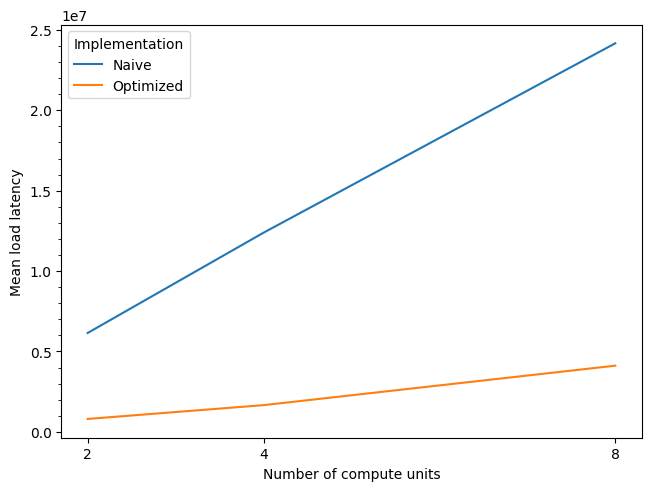
\includegraphics[width=0.6\linewidth]{images/task1/rs4-t1-mean-load-latency.png}
    \caption{Mean load latency across three different configurations for two implementations of the histogram computation kernels.}
    \label{fig:task1:mean-load-latency}
\end{figure}

The \texttt{vALUInsts}, or the average number of executed vector ALU instructions, scale similarly between the naive and optimized implementations. However, the optimized version consistently shows a small but steady increase in instruction count across all compute unit configurations. Both kernels perform the same histogram computation, so the number of vector ALU operations stays roughly the same. The optimized version's higher count of operations is due to the memory privatization overhead when handling private histograms and merging them afterwards. Interestingly, the total number of vector ALU instructions decreases as the number of compute units increases. This is because GEM5 reports the average per compute unit, and with more units available, the work is more evenly distributed, reducing the number of required instructions per unit over time. We also notice a sharper drop in \texttt{vALUInsts} from 2 to 4 compute units, compared to 4 to 8. This reflects the fact that most of the performance gains from parallelization are realized early, suggesting a less efficient execution of the algorithm due to overheads like synchronization when handling private histograms and the merge at the end. This is shown in figure~\ref{fig:task1:alu-instructions}.

\begin{figure}[htbp]
    \centering
    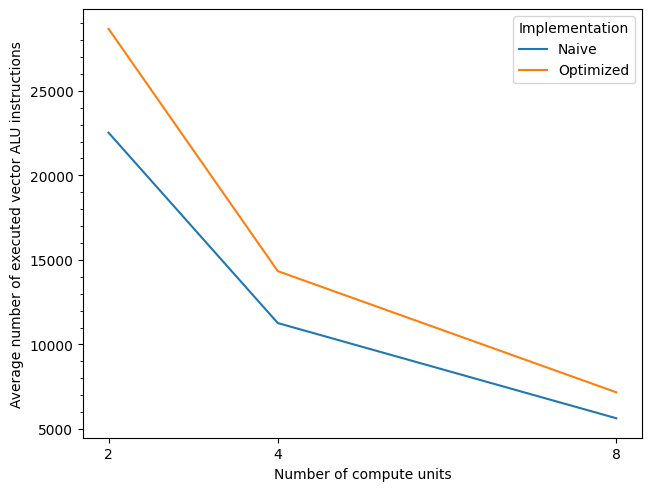
\includegraphics[width=0.6\linewidth]{images/task1/rs4-t1-avg-executed-vector-alu-instructions.png}
    \caption{Average number of executed vector ALU instructions across three different configurations for two implementations of the histogram computation kernels.}
    \label{fig:task1:alu-instructions}
\end{figure}

The \texttt{groupReads} and \texttt{groupWrites} values—representing the average number of reads and writes to shared memory—as well as \texttt{ldsBankAccess}, which tracks the average number of accesses to shared memory banks, all remain consistently zero across all configurations. This is completely expected, as the naive version does not utilize shared memory; instead, all threads directly update a single global histogram in global memory. As a result, there is no accesses to the group segment, and the shared memory traffic remains zero.
The optimized version does show a non-zero value across all configurations. There is a decreasing trend in the number of shared memory access as the number of compute units increases. This trend is consistent across \texttt{groupReads}, \texttt{groupWrites}, and \texttt{ldsBankAccess}, with the number of reads and writes always being equal. This behavior reflects how the workload is divided across more compute units—each unit handles fewer thread groups, leading to fewer shared memory accesses per unit on average. This is shown in figure~\ref{fig:task1:shared-memory}.

\begin{figure*}[htbp]
    \centering
    \subfloat[Average number of accesses of shared memory across three different configurations for two implementations of the histogram computation kernels.]{%
        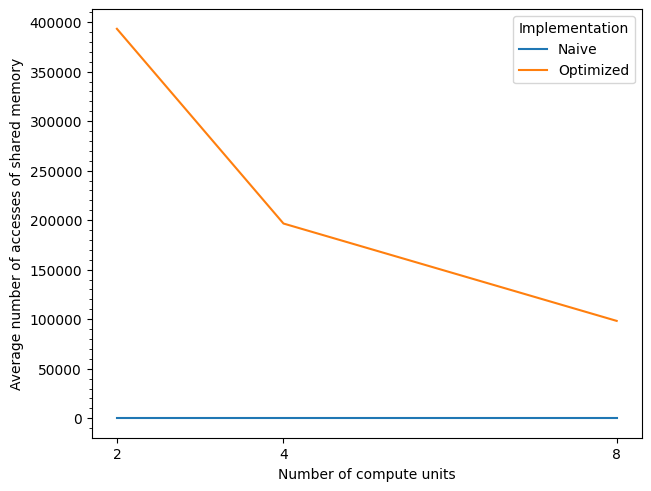
\includegraphics[width=0.6\linewidth]{images/task1/rs4-t1-avg-accesses-of-shared-memory.png}
        \label{fig:task1:shared-accesses}
    }\hfill\\
    
    \subfloat[Average number of reads from shared memory across three different configurations for two implementations of the histogram computation kernels.]{%
        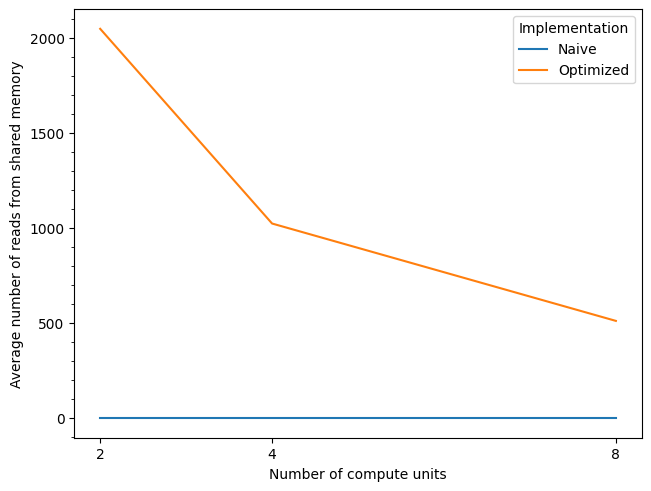
\includegraphics[width=0.4\linewidth]{images/task1/rs4-t1-avg-reads-from-shared-memory.png}
        \label{fig:task1:shared-reads}
    }\hfill
    \subfloat[Average number of writes to shared memory across three different configurations for two implementations of the histogram computation kernels.]{%
        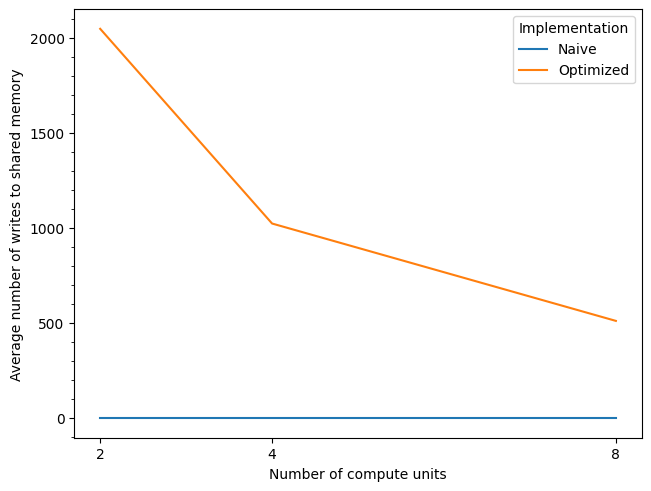
\includegraphics[width=0.4\linewidth]{images/task1/rs4-t1-avg-writes-to-shared-memory.png}
        \label{fig:task1:shared-writes}
    }\\
    
    \caption{Results of the memory accesses for our benchmark.}
    \label{fig:task1:shared-memory}
\end{figure*}

When analyzing \texttt{totalCycles} or the average number of cycles, we observe that the naive implementation consistently performs significantly worse than the optimized version across all configurations. Although there is a slight linear decrease in cycles as we increase compute units from 2 to 4 and from 4 to 8, the improvement is minimal—indicating that memory contention in the naive version severely limits scalability. In contrast, the optimized version shows a much more substantial reduction in total cycles when increasing from 2 to 4 compute units, dropping from approximately 240,000 to 200,000 cycles. However, beyond 4 compute units, the benefit levels off, with the cycle count remaining nearly constant at around 200,000. This suggests that most of the gains from parallelism are largely achieved by the time we reach 4 compute units. Beyond that point, further scaling yields diminishing returns, likely due to overheads such as the merging of privatized histograms, which begin to offset the benefits of increased parallelism. This is shown in figure~\ref{fig:task1:avg-cycles}.

\begin{figure}[htbp]
    \centering
    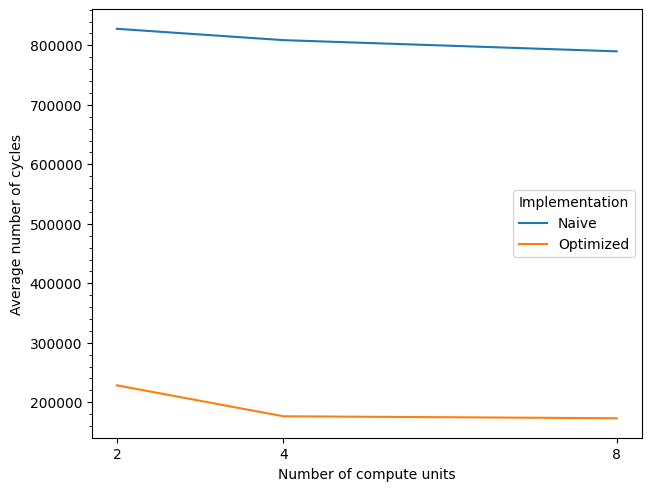
\includegraphics[width=0.6\linewidth]{images/task1/rs4-t1-avg-cycles.png}
    \caption{Average number of cycles across three different configurations for two implementations of the histogram computation kernels.}
    \label{fig:task1:avg-cycles}
\end{figure}

Lastly, let’s look at \texttt{vpc}, or the average number of vector instructions executed per cycle, which directly reflects how efficiently the GPU’s vector processing units are utilized. This tells us how efficiently the GPU's vector processing units are being used. A higher \texttt{vpc} indicates that the GPU is performing more useful computation each cycle, while a lower value suggests it is spending more time stalling—often due to memory access delays.
The results show clearly better computational efficiency for the optimized implementation compared to the naive one across all configurations. While the naive version consistently maintains low \texttt{vpc} values due to memory contention, its decline with increasing compute units stays relatively modest. In contrast, the optimized version starts with a high \texttt{vpc} at 2 CUs but sees a significant drop as compute units increase. This steeper decline is likely due to merging overhead and increased synchronization costs. In both versions, the decrease in \texttt{vpc} is more pronounced from 2 to 4 CUs than from 4 to 8 CUs, suggesting that parallel efficiency starts to degrade at 4 CUs. This is shown in figure~\ref{vpc}.

\begin{figure}[htbp]
    \centering
    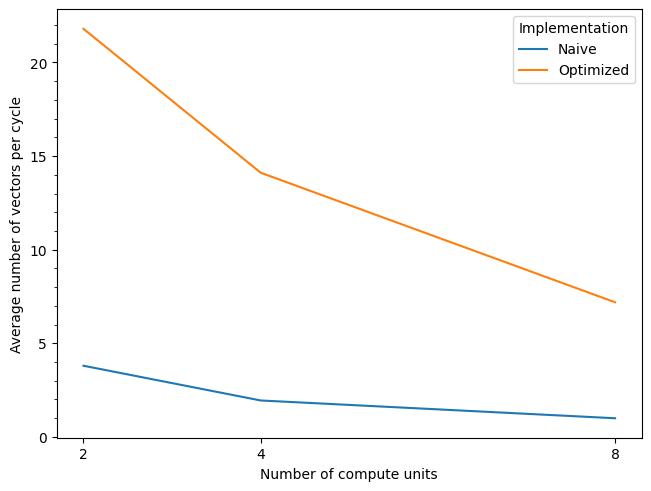
\includegraphics[width=0.6\linewidth]{images/task1/rs4-t1-avg-vectors-per-cycle.png}
    \caption{Average number of vector per cycles across three different configurations for two implementations of the histogram computation kernels.}
    \label{fig:task1:vpc}
\end{figure}

\end{document}
